\section{Results}

\sectioncover

\subsection{Structured mesh}

\begin{frame}
    \begin{columns}
        \begin{column}{0.4\textwidth}
            \begin{figure}
                \centering
                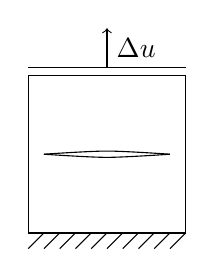
\begin{tikzpicture}[scale=2]
                    \draw (0,0) rectangle (1,1);
                    \draw (0,-0.1) -- (0.1,0);
                    \draw (0.1,-0.1) -- (0.2,0);
                    \draw (0.2,-0.1) -- (0.3,0);
                    \draw (0.3,-0.1) -- (0.4,0);
                    \draw (0.4,-0.1) -- (0.5,0);
                    \draw (0.5,-0.1) -- (0.6,0);
                    \draw (0.6,-0.1) -- (0.7,0);
                    \draw (0.7,-0.1) -- (0.8,0);
                    \draw (0.8,-0.1) -- (0.9,0);
                    \draw (0.9,-0.1) -- (1,0);
                    \draw (0,1.05) -- (1,1.05);
                    \draw[->] (0.5,1.05) -- (0.5,1.3) node[midway,right]{$\Delta u$};
                    \draw plot[smooth] coordinates {(0.1,0.5) (0.5,0.48) (0.9,0.5)};
                    \draw plot[smooth] coordinates {(0.1,0.5) (0.5,0.52) (0.9,0.5)};
                \end{tikzpicture}
            \end{figure}
            \begin{itemize}
                \item[] Parameters
                    \begin{itemize}
                        \item Domain $\Omega = [0, 1]^2$
                        \item Young's modulus $E = 1$
                        \item Poisson's ratio $\nu = 0.3$
                        \item Crack length $a = 0.8$
                        \item Phase field reg. length $l = 0.025$
                        \item Displacement $\Delta u = 0.01$
                        \item Penalty parameter $\alpha = 1$
                    \end{itemize}
            \end{itemize}
        \end{column}
        \vrule{}
        \begin{column}{0.6\textwidth}
            \begin{figure}
                \centering
                \begin{subfigure}{0.32\textwidth}
                    \centering
                    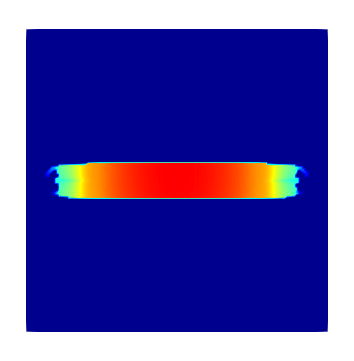
\includegraphics[width=\textwidth]{results/figures/structured_w_4.png}
                    \caption{$l/h = 4$}
                \end{subfigure}
                \begin{subfigure}{0.32\textwidth}
                    \centering
                    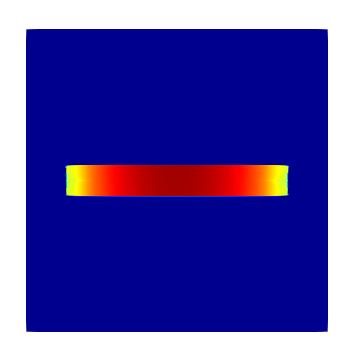
\includegraphics[width=\textwidth]{results/figures/structured_w_8.png}
                    \caption{$l/h = 8$}
                \end{subfigure}
                \begin{subfigure}{0.32\textwidth}
                    \centering
                    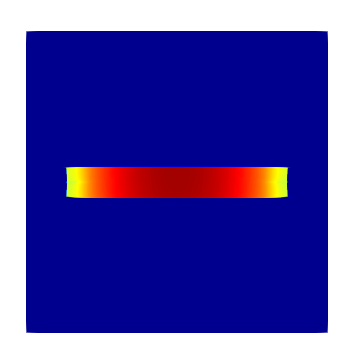
\includegraphics[width=\textwidth]{results/figures/structured_w_16.png}
                    \caption{$l/h = 16$}
                \end{subfigure}
            \end{figure}
        \end{column}
    \end{columns}
\end{frame}

\subsection{Unstructured mesh}

\begin{frame}
\end{frame}

\subsection{Thermal contact -- a patch test}

\begin{frame}
\end{frame}

\subsection{Thermal contact -- comparison to sharp crack solution}

\begin{frame}
\end{frame}